\documentclass[aspectratio=169]{beamer}
\setbeamertemplate{navigation symbols}{}
\usepackage{color, amsmath, comment, subfigure}
\usepackage{url}

\usepackage{hyperref}
\hypersetup{
    colorlinks=true,
    linkcolor=blue,
    filecolor=magenta,      
    urlcolor=cyan,
}

%%%%%%%%%%%%%%%%%%%%%%%%%%
\title[]{Comments slides for Thursday, Oct 15:\\Measuring predictability}
\author[]{Matthew J. Salganik}
\institute[]{}
\date[]{COS 597E/SOC 555 Limits to prediction\\Fall 2020, Princeton University}

\begin{document}
%%%%%%%%%%%%%%%%%%%%%%%%%%%
\frame{\titlepage}
%%%%%%%%%%%%%%%%%%%%%%%%%%%
\begin{frame}
\frametitle{}

Observations/comments/questions/provocations:
\begin{itemize}
\item I'm surprised at how non-systematized this is. Measure of ``predictability'' seem more complex than measure of ``inequality''.
\end{itemize}

\end{frame}
%%%%%%%%%%%%%%%%%%%%%%%%%%%
\begin{frame}
\frametitle{}

\begin{center}
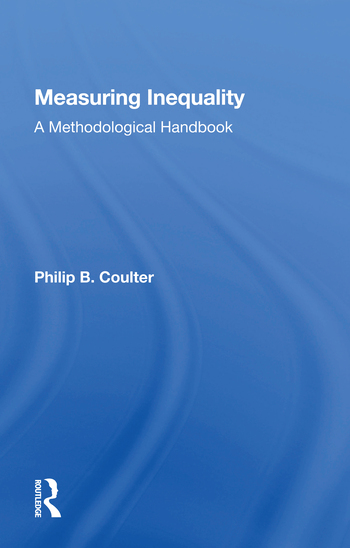
\includegraphics[height=0.8\textheight]{figures/coulter_measuring_1989_cover}
\end{center}

\end{frame}
%%%%%%%%%%%%%%%%%%%%%%%%%%%
\begin{frame}
\frametitle{}

\begin{center}
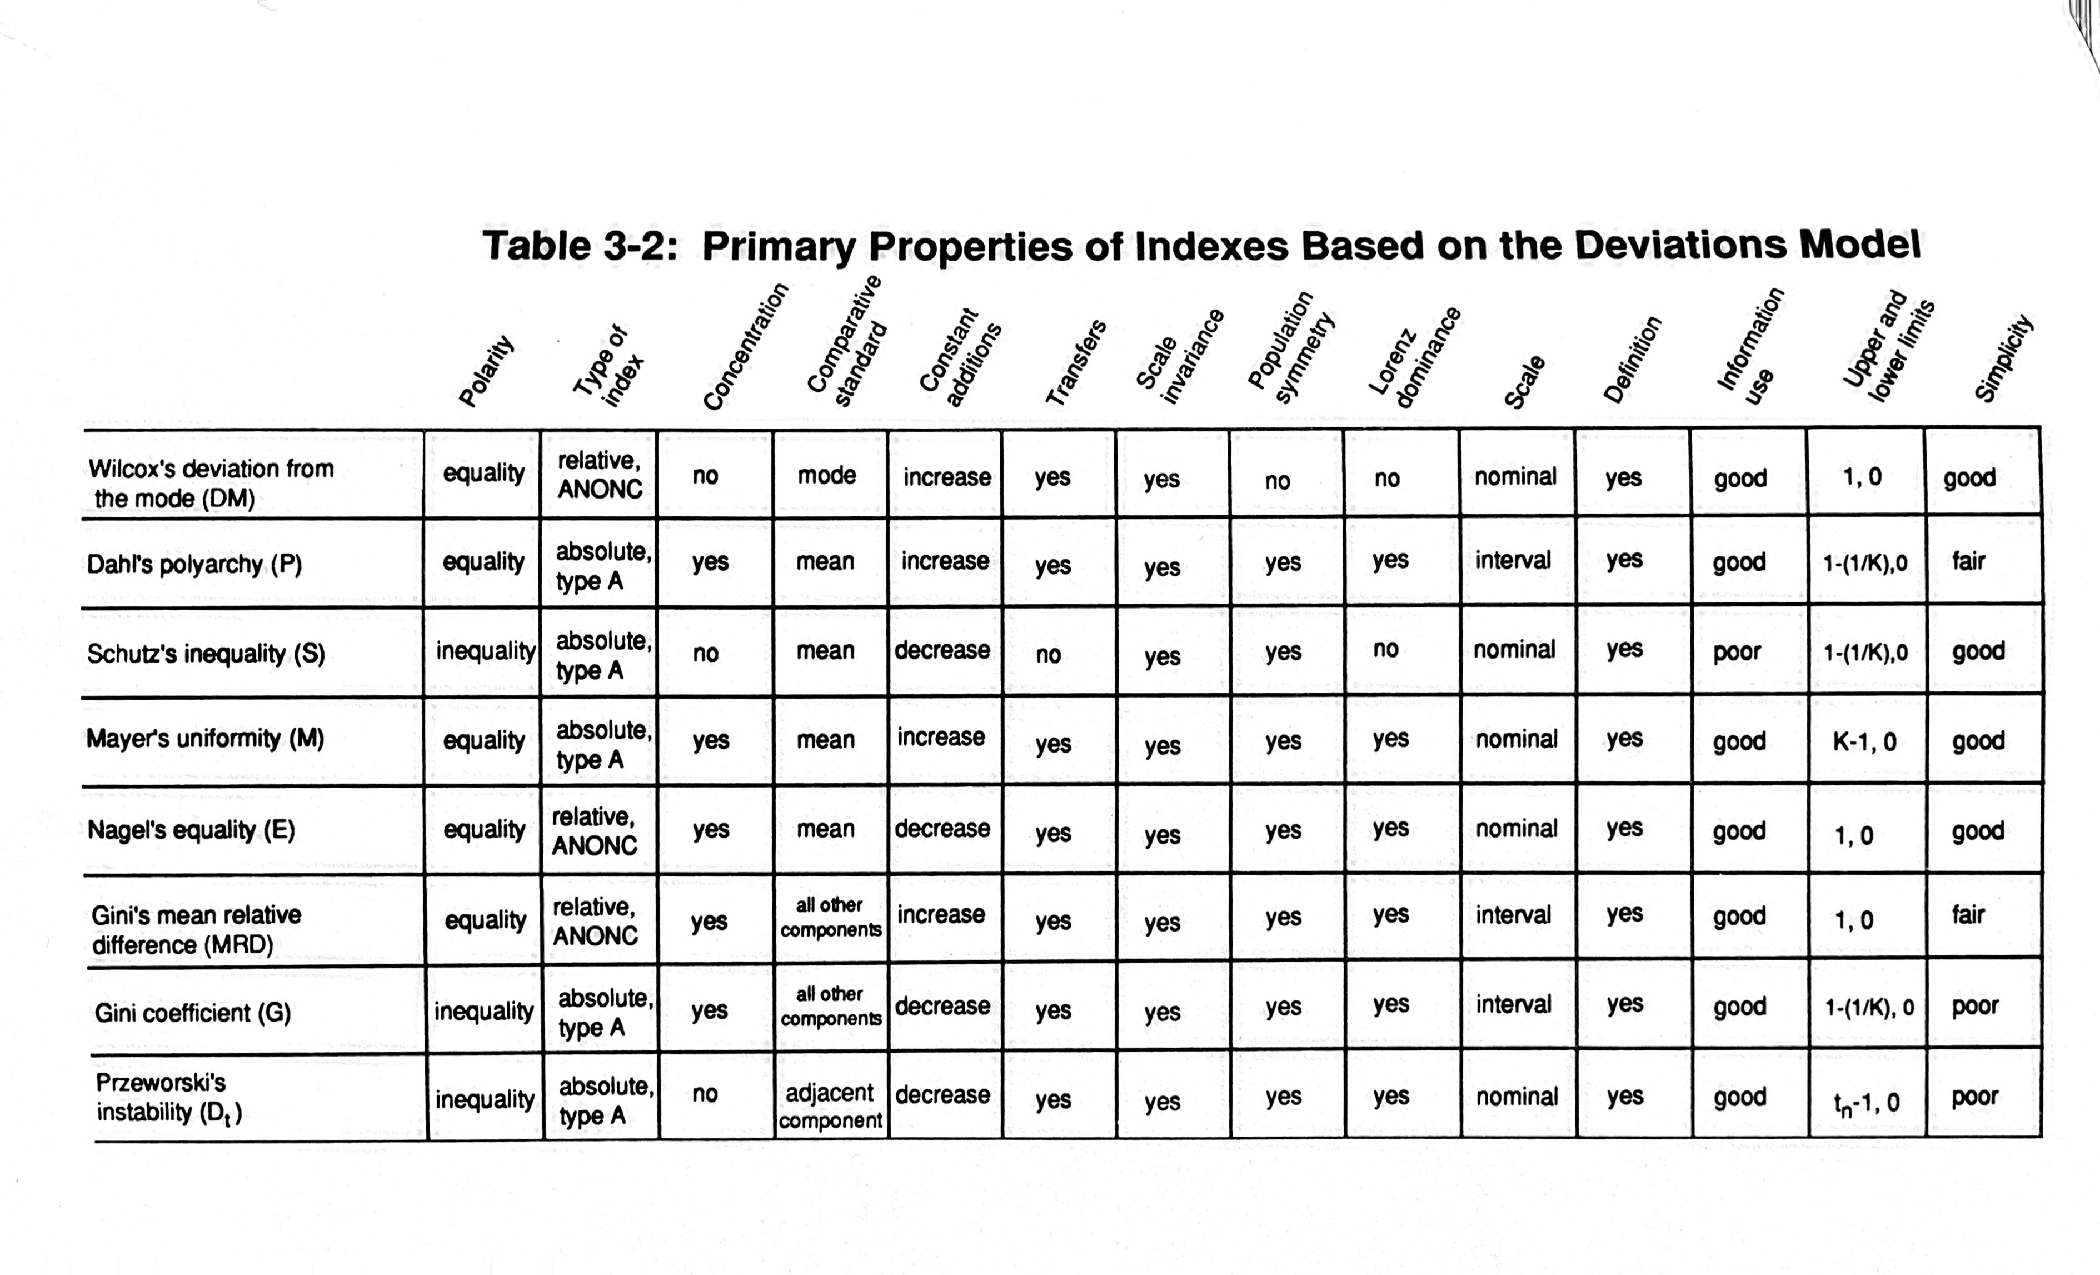
\includegraphics[width=\textwidth]{figures/coulter_measuring_1989_tab3_2}
\end{center}

\end{frame}
%%%%%%%%%%%%%%%%%%%%%%%%%%%
\begin{frame}
\frametitle{}

\begin{center}
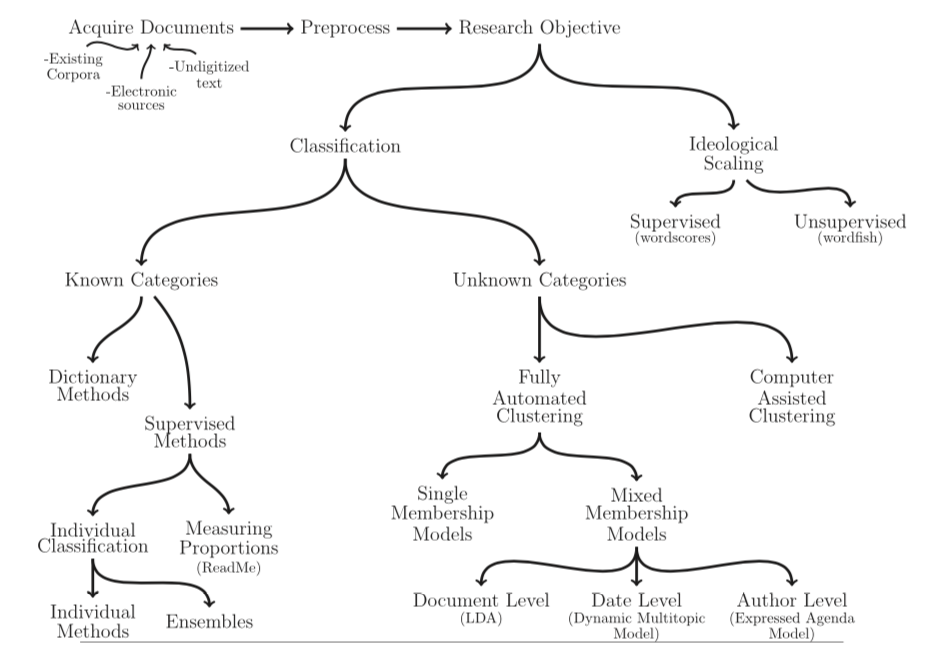
\includegraphics[width=0.6\textwidth]{figures/grimmer_text_2013_fig1}
\end{center}

\end{frame}
%%%%%%%%%%%%%%%%%%%%%%%%%%%
\begin{frame}
\frametitle{}

Observations/comments/questions/provocations:
\begin{itemize}
\item I'm surprised at how non-systematized this is. Measure of ``predictability'' seem more complex than measure of ``inequality''.
\pause
\item We didn't talk any about measure of ``unpredictability''
\pause
\item Single number summaries lose information and hide heterogeneity
\pause
\item $R^2_{Holdout}$ and $MSE_{Holdout}$ are very different
\pause
\item picking a metric because it is ``famous'' can be dangerous, but picking a metric that is not standard can be weird too
\pause
\item For policy we care about ranks and for science we care about values! Maybe?
\pause
\item Classification problems are rare in sociology because we are rarely trying to do anything
\pause
\item Imagine statistical learning produces and uncalibrated score $\tilde{y}$.  Higher $\tilde{y}$ means more likely to get evicted.   We want $\hat{y} = f(\tilde{y})$.  We can learn $f()$. \url{https://machinelearningmastery.com/probability-calibration-for-imbalanced-classification/}. Platt scaling aka Platt calibration. Could this work for continuous outcomes too? How could it?
\end{itemize}

\end{frame}
%%%%%%%%%%%%%%%%%%%%%%%%%%%
\begin{frame}

\begin{center}
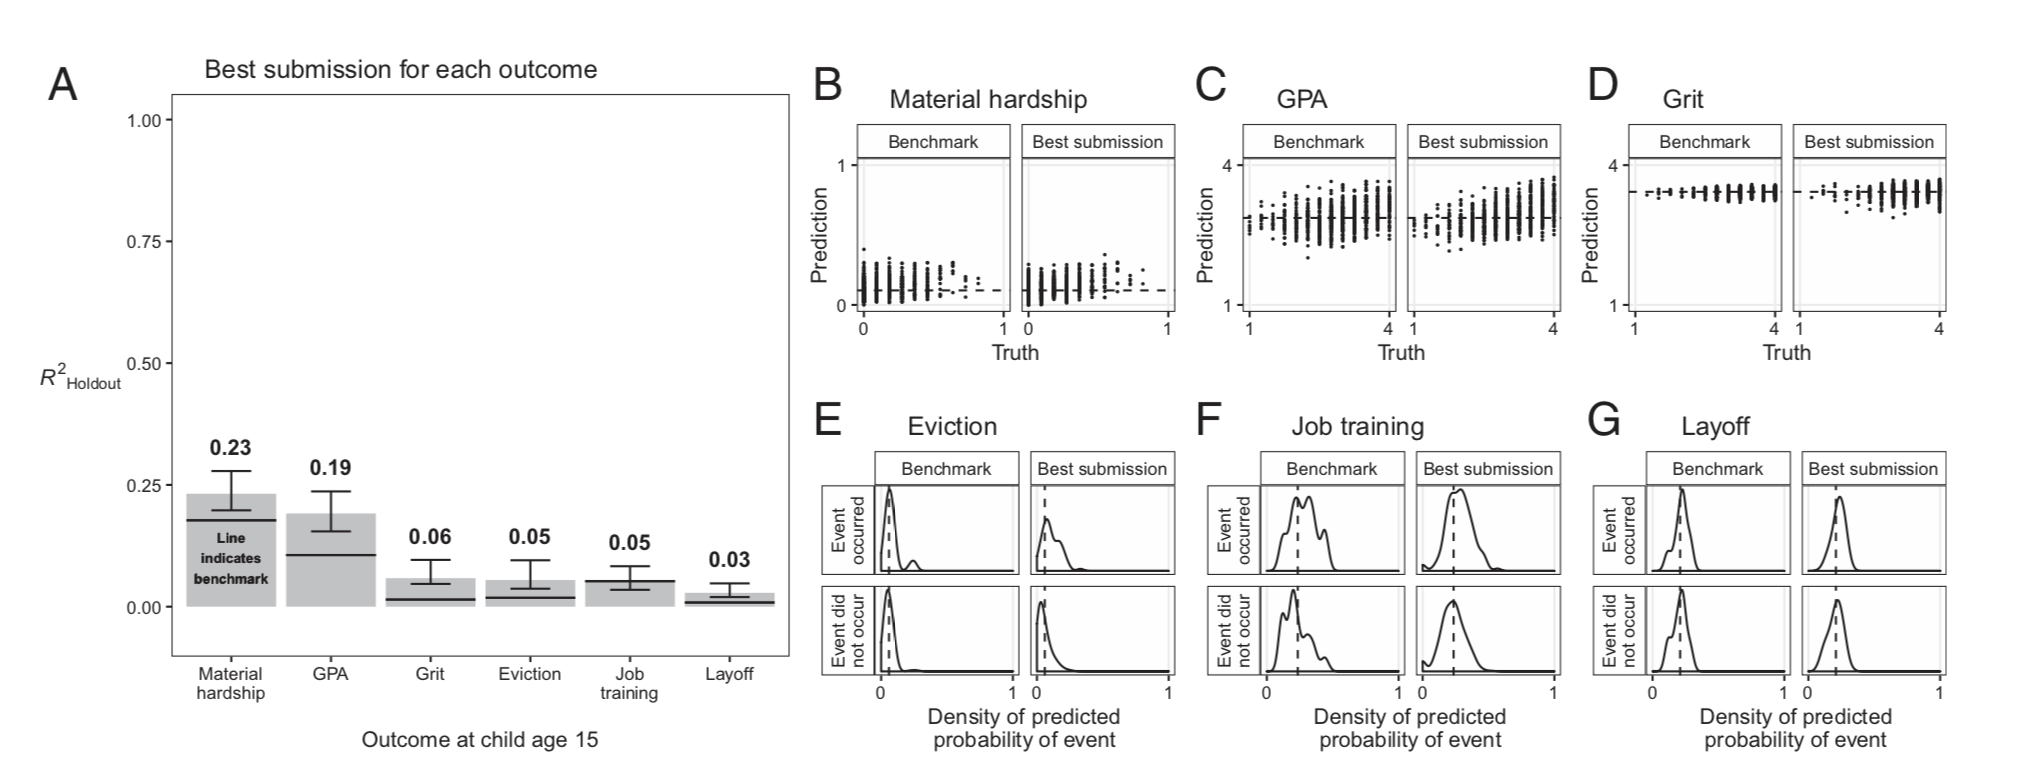
\includegraphics[width=\textwidth]{figures/salganik_measuring_2020_fig2}
\end{center}

\end{frame}
%%%%%%%%%%%%%%%%%%%%%%%%%%%
\begin{frame}

\begin{center}
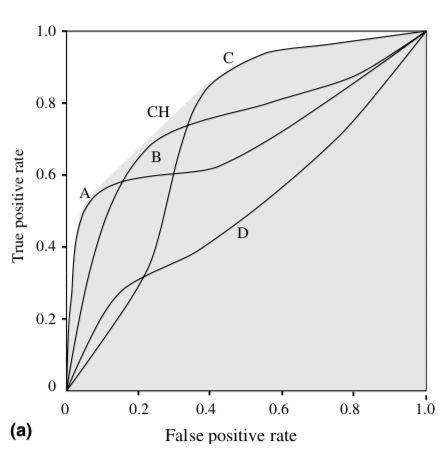
\includegraphics[width=0.6\textwidth]{figures/fawcett_introduction_2006_fig7a}
\end{center}

\end{frame}
%%%%%%%%%%%%%%%%%%%%%%%%%%%
\frame{\titlepage}


\end{document}
